\documentclass[11pt,spanish,a4paper]{article}
% Versión 2.o cuat 2015 Víctor Bettachini < bettachini@df.uba.ar >

\usepackage{babel}
\addto\shorthandsspanish{\spanishdeactivate{~<>}}
\usepackage[utf8]{inputenc}
\usepackage{float}

\usepackage{units}
\usepackage[separate-uncertainty=true, multi-part-units=single, locale=FR]{siunitx}

\usepackage{amsmath}
\usepackage{amstext}
\usepackage{amssymb}

\newcommand{\pvec}[1]{\vec{#1}\mkern2mu\vphantom{#1}}

% \usepackage{tikz}
% \input{DimLinesTikz}
% \usetikzlibrary{decorations.pathmorphing, patterns}

\usepackage{graphicx}
\graphicspath{{./graphs/}}

\usepackage[margin=1.4cm,nohead]{geometry}
% \voffset-3.5cm
% \hoffset-3cm
% \setlength{\textwidth}{17.5cm}
% \setlength{\textheight}{27cm}

\usepackage{lastpage}
\usepackage{fancyhdr}
\pagestyle{fancyplain}
\fancyhead{}
\fancyfoot{{\tiny \textcopyright Departamento de Física, FCEyN, UBA}}
\fancyfoot[C]{ {\tiny Actualizado al \today} }
\fancyfoot[RO, LE]{Pág. \thepage/\pageref{LastPage}}
\renewcommand{\headrulewidth}{0pt}
\renewcommand{\footrulewidth}{0pt}

% \def \materia {Física II para químicos}
\def \periodo {cuatrimestre de verano - 2017}
\def \website {http://materias.df.uba.ar/f2qa2017v}


\begin{document}
\noindent
\textbf{Física II (Químicos)}\hfill \textcopyright {\tt DF, FCEyN, UBA}
% \textbf{\materia}\hfill \periodo
\begin{center}
  \textsc{\large Corrientes variables - Ley de Faraday - Ley de Lenz - Inductancia - Transitorios} 
  % \textsc{\large Guía 5: Corrientes variables - Ley de Faraday - Ley de Lenz - Inductancia - Transitorios} 
\par\end{center}{\large \par}


\begin{enumerate}

\section*{Corrientes variables - Ley de Faraday - Ley de Lenz}
	\item Una espira circular de \(1000\) vueltas y \SI{100}{\centi\metre\squared} de área está colocada en un campo magnético uniforme de \SI{0.01}{T} y rota \(10\) veces por segundo en torno de uno de sus diámetros que es normal a la dirección del campo. Calcular:
	\begin{enumerate}
		\item la f.e.m. inducida en la espira en función del tiempo y, en particular, cuando su normal forma un ángulo de \SI{45}{\degree} con el campo, 
		\item la f.e.m. máxima y mínima y los valores de \(t\) para que aparezcan estas f.e.m.
	\end{enumerate}


	\item \begin{minipage}[t][3.5cm]{0.7\textwidth}
		En la figura se muestra un disco de Faraday, consistente en un disco de cobre de radio \(a\) cuyo eje es paralelo a un campo magnético uniforme \(\vec{B}\).
		Si el disco rota con una velocidad angular \(\omega \), calcular la f.e.m. que aparece entre los puntos \(A\) y \(C\).
    \end{minipage}
    \begin{minipage}[c][1em][t]{0.25\textwidth}
		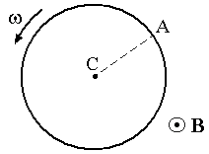
\includegraphics[width=\textwidth]{p5e02}
    \end{minipage}


	\item Los rieles de una vía están separados por \SI{1.5}{\metre} y están aislados entre sí.
		Se conecta entre ellos un milivoltímetro.
		¿Cuánto indica el instrumento cuando pasa un tren a \SI{200}{\kilo\metre\per\hour}?
		Suponer que la componente vertical del campo magnético de la Tierra mide allí \SI{1.5e-5}{\tesla}.


	\item \begin{minipage}[t][3.5cm]{0.65\textwidth}
		Un cable rectilíneo muy largo conduce una corriente \(I\) de \SI{1}{\ampere}.
		A una distancia \(L = \SI{1}{\metre}\) del cable se encuentra el extremo de una aguja de \SI{40}{\centi\metre} de largo que gira en torno de ese extremo en el plano del cable, con una velocidad angular \(\omega = \SI{20\pi}{\per\second}\), como se muestra en la figura.
		Calcular la f.e.m. inducida en los extremos de la aguja como función del tiempo.
    \end{minipage}
    \begin{minipage}[c][1em][t]{0.3\textwidth}
		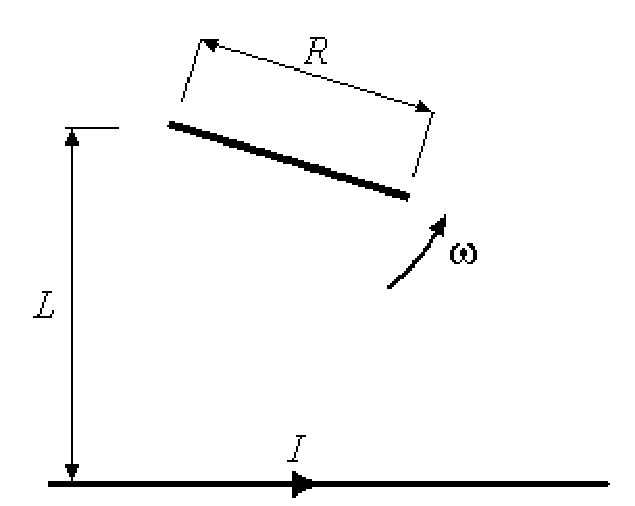
\includegraphics[width=\textwidth]{p5e04}
    \end{minipage}


\section*{Inductancia}
	\item Un solenoide tiene \(1000\) vueltas, \SI{20}{\centi\metre} de diámetro y \SI{40}{\centi\metre} de largo.
		En su centro se ubica otro solenoide de \(100\) vueltas, \SI{4}{\centi\metre} de diámetro y espesor despreciable, cuya resistencia vale \SI{50}{\ohm}.
		Si la corriente que circula por el solenoide exterior aumenta a razón de \SI{0.5}{\ampere} cada \SI{0.2}{\second}, calcular la corriente que se induce en el solenoide interior, cuya autoinductancia es de \SI{2.4}{\milli\henry}.


	\item Calcular la inductancia de\hfill
		\begin{enumerate}
			\item un solenoide infinito de radio \(R\) y \(n\) vueltas por unidad de longitud (exprese el resultado por unidad de longitud),
			\item un toroide con \(N\) vueltas, sección \(S\) y radio medio \(R\), asumiendo que la diferencia entre el radio exterior e interior es mucho menor que \(R\), 
			\item y un solenoide con \(N\) vueltas de longitud \(L\) y radio \(R\) (suponga \(R \ll L\).
		\end{enumerate}


	\item Calcule la energía magnética por unidad de longitud para el cable coaxial del Problema \(10\) de la Guía \(4\).
		Utilizando la relación entre la energía y la autoinductancia, encuentre esta última.


	\item Dos cables rectilíneos paralelos de radio \(r\), separados por una distancia \(d\), pueden suponerse como un circuito que se cierra por el infinito.
		Encuentre la autoinductancia por unidad de longitud cuando \(r \ll d\).


	\item Calcule \(M_{12}\) y \(M_{21}\) entre una espira circular de radio \(R\) y un solenoide finito de longitud \(L\) y radio \(r\) (suponga \(r \ll L\) y \(r \ll R\)), dispuestos de tal forma que los centros y los ejes de ambos son coincidentes.
		Utilice las aproximaciones que crea necesarias y diga cuál de los dos resultados es más confiable cuando \(L\) es pequeño respecto a \(R\).


	\item Dos bobinas están conectadas en serie a una distancia tal que la mitad del flujo de una de ellas atraviesa también la otra.
		Si la autoinducción de las bobinas es \(L\), calcular la autoinducción del conjunto, suponiendo que las bobinas están conectadas de tal forma que los flujos se suman.


\section*{Transitorios}
	\item Un condensador de \SI{3}{\micro\farad} se carga a \SI{271.8}{\volt} y luego se descarga a través de una resistencia de \SI{1}{\mega\ohm}.
		Calcular:
		\begin{enumerate}
			\item el voltaje sobre el condensador luego de 3 segundos, 
			\item y el calor disipado en la resistencia durante la descarga completa del condensador.
		\end{enumerate}
	Compare el último resultado con la energía almacenada en el condensador al comienzo de la descarga.


	\item \begin{minipage}[t]{0.6\textwidth}
		La figura muestra las condiciones del circuito antes de \(t= 0\), instante en que se cierra la llave \(S\).
		Calcular para todo \(t> 0\):
		\begin{enumerate}
			\item el voltaje sobre el condensador \(C_2\),
			\item y la corriente.
		\end{enumerate}
    \end{minipage}
    \begin{minipage}[c][1em][t]{0.35\textwidth}
		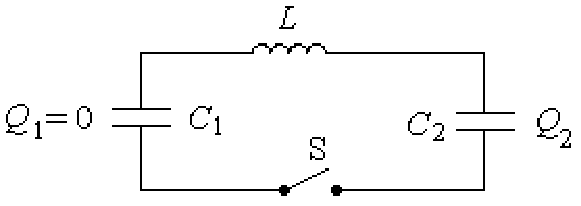
\includegraphics[width=\textwidth]{p5e12}
    \end{minipage}


	\item Una f.e.m. de \SI{400}{\volt} se conecta en tiempo \(t= 0\) a un circuito serie formado por una inductancia \(L= \SI{2}{\henry}\), una resistencia \(R= \SI{20}{\ohm}\) y un capacitor \(C= \SI{8}{\micro\farad}\) inicialmente descargado.
		\begin{enumerate}
			\item Demostrar que el proceso de carga es oscilatorio, calcular la frecuencia de las oscilaciones y compárela con el valor de \(\frac{1}{\sqrt{LC}}\).
			\item Calcular la derivada temporal inicial de la corriente.
			\item Hallar, en forma aproximada, la máxima tensión sobre \(C\).
			\item ¿Qué resistencia debe agregarse en serie para que el amortiguamiento del circuito sea crítico?
		\end{enumerate}


	\item \begin{minipage}[t]{0.65\textwidth}
		En el circuito que se muestra en la figura todas las resistencias son iguales.
		En el instante \(t_0= 0\) se cierra la llave que conecta al capacitor que se encuentra descargado.
		Calcule el tiempo que demanda alcanzar al capacitor el \(99\%\) de su carga máxima e indique cuál será su polaridad.
    \end{minipage}
    \begin{minipage}[c][1em][t]{0.3\textwidth}
		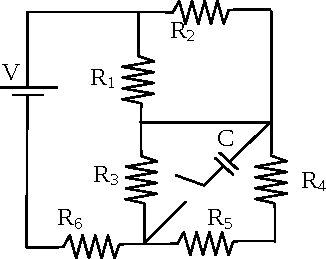
\includegraphics[width=\textwidth]{p5e14}
    \end{minipage}



\end{enumerate}
% \end{description}
\end{document}
